\documentclass[11pt]{article}
\usepackage[a4paper,margin=1in]{geometry}
\usepackage{amsmath,amssymb}
\usepackage[T1]{fontenc}
\usepackage{lmodern}
\usepackage{microtype}
\usepackage{xcolor}
\usepackage{footnote}
\usepackage{tikz}
\usetikzlibrary{arrows.meta,positioning,calc}

\setlength{\parindent}{0pt}
\setlength{\parskip}{0.5em}

\newcommand{\promptbox}[1]{%
  \begin{savenotes}%
  \begingroup\setlength{\fboxsep}{10pt}\noindent
  \colorbox{blue!8}{\parbox{\dimexpr\linewidth-2\fboxsep\relax}{\textbf{Prompt. }#1}}
  \endgroup
  \end{savenotes}%
}
\newcommand{\resultbox}[1]{%
  \begin{savenotes}%
  \begingroup\setlength{\fboxsep}{10pt}\noindent
  \colorbox{purple!8}{\parbox{\dimexpr\linewidth-2\fboxsep\relax}{\textbf{Result. }#1}}
  \endgroup
  \end{savenotes}%
}
\newcommand{\examplebox}[1]{%
  \begin{savenotes}%
  \begingroup\setlength{\fboxsep}{10pt}\noindent
  \colorbox{green!8}{\parbox{\dimexpr\linewidth-2\fboxsep\relax}{\textbf{Example. }#1}}
  \endgroup
  \end{savenotes}%
}

\title{\textbf{Book 1 --- Lecture 2 --- Exercise 4}\\[2mm]
\large Proving the Sum, Product, and Chain Rules}
\author{}
\date{}

\begin{document}
\maketitle

\promptbox{Prove the sum rule (fairly easy), the product rule (easy if you know
the trick), and the chain rule (fairly easy).\footnote{Throughout, work at a fixed
point \(x\) in an open interval where the functions written are differentiable in
the usual real sense. Limits are taken as \(h\to 0\) with \(h\neq 0\).}}

\section*{Setup}
Let \(f\) and \(g\) be differentiable at \(x\).\footnote{The \emph{derivative at
\(x\)} is \(f'(x)=\lim_{h\to 0}\dfrac{f(x+h)-f(x)}{h}\) when this limit exists.}

\section*{Sum rule}
Define \(S=f+g\). For \(h\neq 0\),
\[
\frac{S(x+h)-S(x)}{h}
=\frac{f(x+h)-f(x)}{h}+\frac{g(x+h)-g(x)}{h}.
\]
Each quotient has a limit as \(h\to 0\) by hypothesis; limits add termwise, so
\[
S'(x)=f'(x)+g'(x).
\]
Equivalently, \((f+g)'=f'+g'\) at each point where both derivatives exist.

\paragraph{Picture (sum).}
Over the \emph{same} step from \(x\) to \(x+h\), the vertical changes in \(f\),
\(g\), and \(S=f+g\) add: \(\Delta S=\Delta f+\Delta g\). Dividing by \(h\) and
letting \(h\to 0\), the secant slopes add the same way the rises do.

\begin{center}
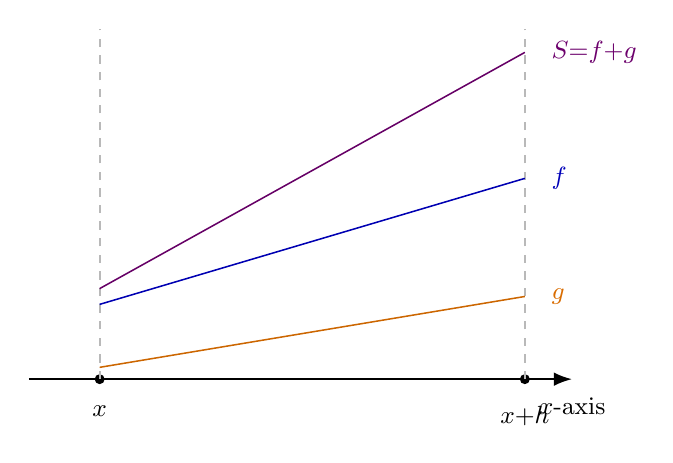
\begin{tikzpicture}[>=Latex, thick, x=1cm, y=1cm]
  \coordinate (x0) at (0.6,0);
  \coordinate (x1) at (6.0,0);
  \coordinate (g0) at ($(x0)+(0,0.15)$);
  \coordinate (g1) at ($(x1)+(0,1.05)$);
  \coordinate (f0) at ($(x0)+(0,0.95)$);
  \coordinate (f1) at ($(x1)+(0,2.55)$);
  \coordinate (s0) at ($(x0)+(0,1.15)$);
  \coordinate (s1) at ($(x1)+(0,4.15)$);
  \draw[-{Latex}] (-0.3,0) -- (6.6,0) node[below=3pt, font=\small]{$x$-axis};
  \fill (x0) circle (1.8pt) node[below=6pt, font=\small]{$x$};
  \fill (x1) circle (1.8pt) node[below=6pt, font=\small]{$x{+}h$};
  \draw[dashed, gray!55] (x0) -- ($(x0)+(0,4.45)$);
  \draw[dashed, gray!55] (x1) -- ($(x1)+(0,4.45)$);
  \draw[orange!80!black, line width=0.55pt] (g0) -- (g1);
  \draw[blue!70!black, line width=0.55pt] (f0) -- (f1);
  \draw[violet!80!black, line width=0.55pt] (s0) -- (s1);
  % labels beside the right endpoints so chords do not cross text
  \node[orange!85!black, font=\small, anchor=west, inner sep=3pt] at ($(g1)+(0.22,0)$) {$g$};
  \node[blue!72!black, font=\small, anchor=west, inner sep=3pt] at ($(f1)+(0.22,0)$) {$f$};
  \node[violet!85!black, font=\small, anchor=west, inner sep=3pt, align=left]
    at ($(s1)+(0.22,0)$) {$S{=}f{+}g$};
\end{tikzpicture}\\[0.55em]
{\small Rises \(\Delta f\), \(\Delta g\) over \([x,x+h]\) stack to \(\Delta S\);
hence \(\dfrac{\Delta S}{h}=\dfrac{\Delta f}{h}+\dfrac{\Delta g}{h}\).}
\end{center}

\section*{Product rule}
Write the Newton quotient for \(P=fg\), then add and subtract the same term
\(f(x+h)g(x)\) in the numerator:\footnote{This ``trick'' isolates increments of \(f\)
holding \(g\) fixed at \(x\), and increments of \(g\) holding a prefactor that
becomes \(f(x)\) as \(h\to 0\) because differentiable functions are continuous.}
\begin{align*}
P(x+h)-P(x)
&=f(x+h)g(x+h)-f(x)g(x)\\
&=f(x+h)\bigl(g(x+h)-g(x)\bigr)+g(x)\bigl(f(x+h)-f(x)\bigr).
\end{align*}
Divide by \(h\neq 0\):
\[
\frac{P(x+h)-P(x)}{h}
=f(x+h)\,\frac{g(x+h)-g(x)}{h}+g(x)\,\frac{f(x+h)-f(x)}{h}.
\]
Let \(h\to 0\). By continuity of \(f\) at \(x\), \(f(x+h)\to f(x)\). Hence
\[
P'(x)=f(x)g'(x)+g(x)f'(x).
\]

\paragraph{Picture (product).}
Think of \(f\) and \(g\) as side lengths of a rectangle, so \(P=fg\) is its
area.\footnote{This is bookkeeping only: \(f\) and \(g\) are abstract quantities;
the picture assumes \(h\) is small enough that both \(f(x{+}h)\) and \(g(x{+}h)\)
lie on the same side of zero as \(f(x)\) and \(g(x)\) so lengths are positive.}
When \(f\) and \(g\) change, the new area splits into the old rectangle plus a
``top strip'' (width \(f(x{+}h)\), height \(\Delta g\)) and a ``right strip''
(height \(g(x)\), width \(\Delta f\)). That is exactly the two grouped terms before
dividing by \(h\).

\begin{center}
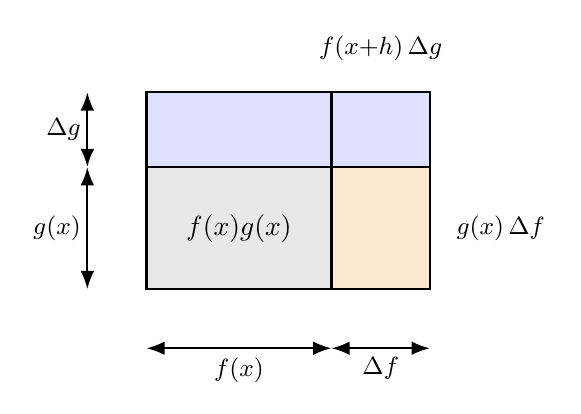
\begin{tikzpicture}[>=Latex, thick, x=1cm, y=1cm]
  % Inner rectangle f(x) x g(x); outer f(x+h) x g(x+h). Positive increments.
  \def\fx{2.35}      % f(x)
  \def\gx{1.55}      % g(x)
  \def\df{1.25}      % Delta f
  \def\dg{0.95}      % Delta g
  \def\dimgap{0.75} % gap for dimension brackets
  \fill[gray!18] (0,0) rectangle (\fx,\gx);
  \fill[blue!12] (0,\gx) rectangle ({\fx+\df},\gx+\dg);
  \fill[orange!18] (\fx,0) rectangle ({\fx+\df},\gx);
  \draw (0,0) rectangle ({\fx+\df},\gx+\dg);
  \draw (\fx,0) -- (\fx,{\gx+\dg});
  \draw (0,\gx) -- ({\fx+\df},\gx);
  \path ({\fx/2},{\gx/2}) node[inner sep=2pt] {$f(x)g(x)$};
  % strip labels outside colored regions (blue above, orange to the right)
  \node[font=\small, anchor=south, inner sep=3pt, align=center]
    at ({\fx+\df/2},{\gx+\dg+0.28}) {$f(x{+}h)\,\Delta g$};
  \node[font=\small, anchor=west, inner sep=3pt]
    at ({\fx+\df+0.22},{\gx/2}) {$g(x)\,\Delta f$};
  \draw[<->] (0,{-\dimgap}) -- node[below=2pt, font=\small, inner sep=1pt] {$f(x)$} (\fx,{-\dimgap});
  \draw[<->] (\fx,{-\dimgap}) -- node[below=2pt, font=\small, inner sep=1pt] {$\Delta f$} ({\fx+\df},{-\dimgap});
  \draw[<->] ({-\dimgap},0) -- node[left, font=\small, inner sep=2pt, align=right] {$g(x)$} ({-\dimgap},\gx);
  \draw[<->] ({-\dimgap},\gx) -- node[left, font=\small, inner sep=2pt, align=right] {$\Delta g$} ({-\dimgap},{\gx+\dg});
\end{tikzpicture}\\[0.55em]
{\small Shaded: original area. Blue strip: \(f(x{+}h)\bigl(g(x{+}h)-g(x)\bigr)\).
Orange strip: \(g(x)\bigl(f(x{+}h)-f(x)\bigr)\). Sum \(=\,P(x{+}h)-P(x)\).}
\end{center}

\section*{Chain rule}
Let \(F=f\circ g\) with \(F(x)=f(g(x))\). Assume \(g\) is differentiable at \(x\) and
\(f\) is differentiable at \(u=g(x)\).\footnote{The composition need not be differentiable
without both hypotheses at the matching points.}

For \(h\neq 0\), define the ``difference quotient for \(f\) along the increment of
\(g\)'' by
\[
Q(h)=
\begin{cases}
\dfrac{f(g(x+h))-f(g(x))}{g(x+h)-g(x)}, & g(x+h)\neq g(x),\\[6pt]
f'(g(x)), & g(x+h)=g(x).
\end{cases}
\]
If \(g(x+h)=g(x)\), then also \(f(g(x+h))-f(g(x))=0\), so \(F(x+h)-F(x)=0\) and
\[
\frac{F(x+h)-F(x)}{h}=0=Q(h)\cdot\frac{g(x+h)-g(x)}{h}.
\]
If \(g(x+h)\neq g(x)\), then directly
\[
\frac{F(x+h)-F(x)}{h}
=Q(h)\cdot\frac{g(x+h)-g(x)}{h}.
\]
So in either case the same product formula holds for all nonzero \(h\).\footnote{This
unifies the \(\Delta u=0\) and \(\Delta u\neq 0\) cases without separate limit arguments.}

Because \(f\) is differentiable at \(u=g(x)\), one has \(Q(h)\to f'(u)\) as \(h\to 0\)
(when \(g(x+h)\neq g(x)\), \(Q(h)\) is the usual secant slope; when \(g(x+h)=g(x)\) it is
already pinned to \(f'(u)\)). Also \(\dfrac{g(x+h)-g(x)}{h}\to g'(x)\). Products pass
through limits, hence
\[
F'(x)=\lim_{h\to 0}Q(h)\cdot\lim_{h\to 0}\frac{g(x+h)-g(x)}{h}=f'(g(x))\,g'(x).
\]

\paragraph{Picture (chain).}
Two stages: an ``inner'' map \(x\mapsto u=g(x)\), then an ``outer'' map
\(u\mapsto f(u)\). A small move \(h\) at \(x\) produces a small change
\(\Delta u\approx g'(x)\,h\) in the intermediate variable; that change, viewed on
the \(u\)-axis, produces \(\Delta F\approx f'(u)\,\Delta u\). Multiplying the
local rates gives \(\Delta F/h\approx f'(u)\cdot g'(x)\). The algebraic \(Q(h)\)
construction is the bookkeeping that makes the \(\Delta u=0\) case match the
same formula.

\begin{center}
\begin{tikzpicture}[
    >=Latex,
    node distance=1.9cm and 2.15cm,
    box/.style={draw, rounded corners=2.5pt, inner sep=7pt, font=\small},
  ]
  \node (x) {\(x\)};
  \node[right=of x, box] (g) {\(g\)};
  \node[right=of g, font=\small, inner sep=2pt] (u) {\(u{=}g(x)\)};
  \node[right=of u, box] (f) {\(f\)};
  \node[right=of f, font=\small, inner sep=2pt] (y) {\(F{=}f(u)\)};
  \draw[->] (x) -- (g);
  \draw[->] (g) -- node[below=4pt, font=\scriptsize, inner sep=1pt] {$\Delta u$} (u);
  \draw[->] (u) -- (f);
  \draw[->] (f) -- node[below=4pt, font=\scriptsize, inner sep=1pt] {$\Delta F$} (y);
  % midpoints between boxes for labels — extra vertical gap avoids edge overlap
  \coordinate (m_inner) at ($(g.east)!0.5!(u.west)$);
  \coordinate (m_outer) at ($(f.east)!0.5!(y.west)$);
  \node[below=1.35cm of m_inner, font=\scriptsize, align=center, text width=3.1cm]
    {inner slope\\[2pt]\(\dfrac{\Delta u}{h}\to g'(x)\)};
  \node[below=1.35cm of m_outer, font=\scriptsize, align=center, text width=3.1cm]
    {outer slope\\[2pt]\(\dfrac{\Delta F}{\Delta u}\to f'(u)\)};
\end{tikzpicture}\\[0.55em]
{\small Overall secant: \(\dfrac{\Delta F}{h}
=\dfrac{\Delta F}{\Delta u}\cdot\dfrac{\Delta u}{h}\) when \(\Delta u\neq 0\);
the piecewise \(Q(h)\) extends this to \(\Delta u=0\).}
\end{center}

\resultbox{For differentiable \(f,g\) at \(x\),
\[
(f+g)'(x)=f'(x)+g'(x),\qquad
(fg)'(x)=f'(x)g(x)+f(x)g'(x).
\]
For \(F=f\circ g\) with \(g\) differentiable at \(x\) and \(f\) differentiable at
\(g(x)\),
\[
(f\circ g)'(x)=f'(g(x))\,g'(x).
\]}

\examplebox{Sum: \((x^2+\sin x)'=2x+\cos x\). Product: \((x\sin x)'=\sin x+x\cos x\).
Chain: \(\dfrac{d}{dx}\sin(x^2)=2x\cos(x^2)\).}

\end{document}
